\documentclass[11pt]{article}
\usepackage{amssymb}

\usepackage[T1]{fontenc}
\usepackage{inconsolata}
\usepackage{textcomp}
\usepackage{listings}
\usepackage{color}
\usepackage[normalem]{ulem}
\usepackage{float}
\usepackage{graphicx}
\usepackage{amsmath}
\usepackage{mathtools}
\graphicspath{ {figs/} }
\usepackage[hidelinks]{hyperref}
\usepackage{xcolor,soul,lipsum}
\newcommand{\myul}[2][black]{\setulcolor{#1}\ul{#2}\setulcolor{black}}
\usepackage{enumitem}
\usepackage[bottom]{footmisc}


\makeatletter
\DeclareUrlCommand\ULurl@@{%
  \def\UrlFont{\ttfamily\color{blue}}%
  \def\UrlLeft{\uline\bgroup}%
  \def\UrlRight{\egroup}}
\def\ULurl@#1{\hyper@linkurl{\ULurl@@{#1}}{#1}}
\DeclareRobustCommand*\ULurl{\hyper@normalise\ULurl@}
\makeatother


\makeatletter
\renewcommand\thesection{}
\renewcommand\thesubsection{}
\makeatother

\textwidth=6in
\oddsidemargin=0.25in
\evensidemargin=0.25in
\topmargin=-0.1in
\footskip=0.8in
\parindent=0.0cm
\parskip=0.3cm
\textheight=8.00in
\setcounter{tocdepth} {3}
\setcounter{secnumdepth} {2}
\sloppy

\begin{document}

\setlength{\oddsidemargin}{.25in}
\setlength{\evensidemargin}{.25in}
\setlength{\textwidth}{6in}
\setlength{\topmargin}{-0.4in}
\setlength{\textheight}{8.5in}

\newcommand{\handout}[5]{
   \renewcommand{\thepage}{#1-\arabic{page}}
   \noindent
   \begin{center}
   \framebox{
      \vbox{
    \hbox to 5.78in { {\bf Reinforcement Learning} \hfill #2 }
       \vspace{4mm}
       \hbox to 5.78in { {\Large \hfill #5  \hfill} }
       \vspace{2mm}
       \hbox to 5.78in { {\it #3 \hfill #4} }
      }
   }
   \end{center}
   \vspace*{4mm}
}
\newcommand{\exercise}[4]{\handout{#1}{#2}{Lecturer:#3}{TA: #4}{Exercise #1}}
\newenvironment{remark}{\noindent{\bf Remark}\hspace*{1em}}{\bigskip}

%%%%%%%%%%%%%%%%%%%%%%%%%%%%%%%%%%%%%%%%%%%%%%%%%%%%%%%%%%%%%%%%%%%%%%%%%%%%%%%%%%%%%

\exercise{1}{February 27, 2022}{Yishay Mansour}{Asaf Cassel}

\lstdefinestyle{myLuastyle}
{
  language         = {[5.2]Lua},
  showstringspaces = false,
  upquote          = true,
  basicstyle=\ttfamily,
  keywordstyle=\color{blue}\ttfamily,
  stringstyle=\color{red}\ttfamily,
  commentstyle=\color{green}\ttfamily,
  morecomment=[l][\color{magenta}]{\#}
}

\lstset{style=myLuastyle}

Due date: March 13, 2022
\section{Introduction}
In this exercise you will:
\begin{enumerate}
	\item Practice basic dynamic programing definitions.
	\item Get familiar with PyTorch by training a simple neural network on a small dataset.
	\item Get familiar with OpenAI gym environment by training an agent using random search. 
\end{enumerate}

\section{Setup}

For the programing section, you will need to setup a python environment containing the following packages: PyTorch and OpenAI Gym.
\begin{itemize}
\item Conda installation
\item PyTorch installation, follow the instruction here: \url{http://pytorch.org/}
\item OpenAI Gym installation, follow the instruction here: \url{https://gym.openai.com/docs/}
\end{itemize}

% In case you are working on Tel-Aviv University servers, the environment is already installed at: \text{\ttfamily{/usr/local/lib/anaconda3-5.1.0/bin/python}}.
\section{Theory}


\subsection{Question 1: Longest Common Subsequence}
Write a dynamic programming solution for the following problem.\\
Given: Two sequences (or strings) $X(1:m)$ and $Y(1:n)$.\\
Goal: Return the length of the longest common subsequence of both $X$ and
$Y$ (not necessarily contiguous).\\
For Example: \\
\centerline{ $X=\underline{A}V\underline{B}V\underline{A}M\underline{CD}$} \\
\centerline{ $Y=\underline{A}Z\underline{B}Q\underline{AC}L\underline{D}$} \\
\centerline{ Answer = $5$}\\

* For full credits, your algorithm should run in time $O(nm)$. 




% \subsection{Question 1: Longest increasing subsequence\protect\footnote{Question taken from ``046194 - Learning and Planning in Dynamical Systems'' by Shie Manor\textcopyright}}

% Given a sequence of $n$ real numbers $a_1, a_2,\dots,a_n$, find the longest strictly increasing subsequence (not necessarily contiguous). \\
% For example, for the sequence $(3, 1, 5, 3, 4)$, the solution is $(1, 3, 4)$.\\
% Remark: the number of subsequences is $2^n$,  therefore an exhaustive search is inefficient.

\subsection{Question 2: Moses the mouse\protect\footnote{Question taken from ``046194 - Learning and Planning in Dynamical Systems'' by Shie Manor\textcopyright}}

Moses the mouse starts his journey at the south west room
in a $M*N$ rectangular apartment with $M*N$ rooms of size $1*1$,  some of which contain
cheese. After his rare head injury in the mid-scroll war, Moses can only travel north or
east. An illustration of Moses's life for $M=5, N=8$  is given in the following figure:  

\begin{figure*}[ht!]
  \centering
  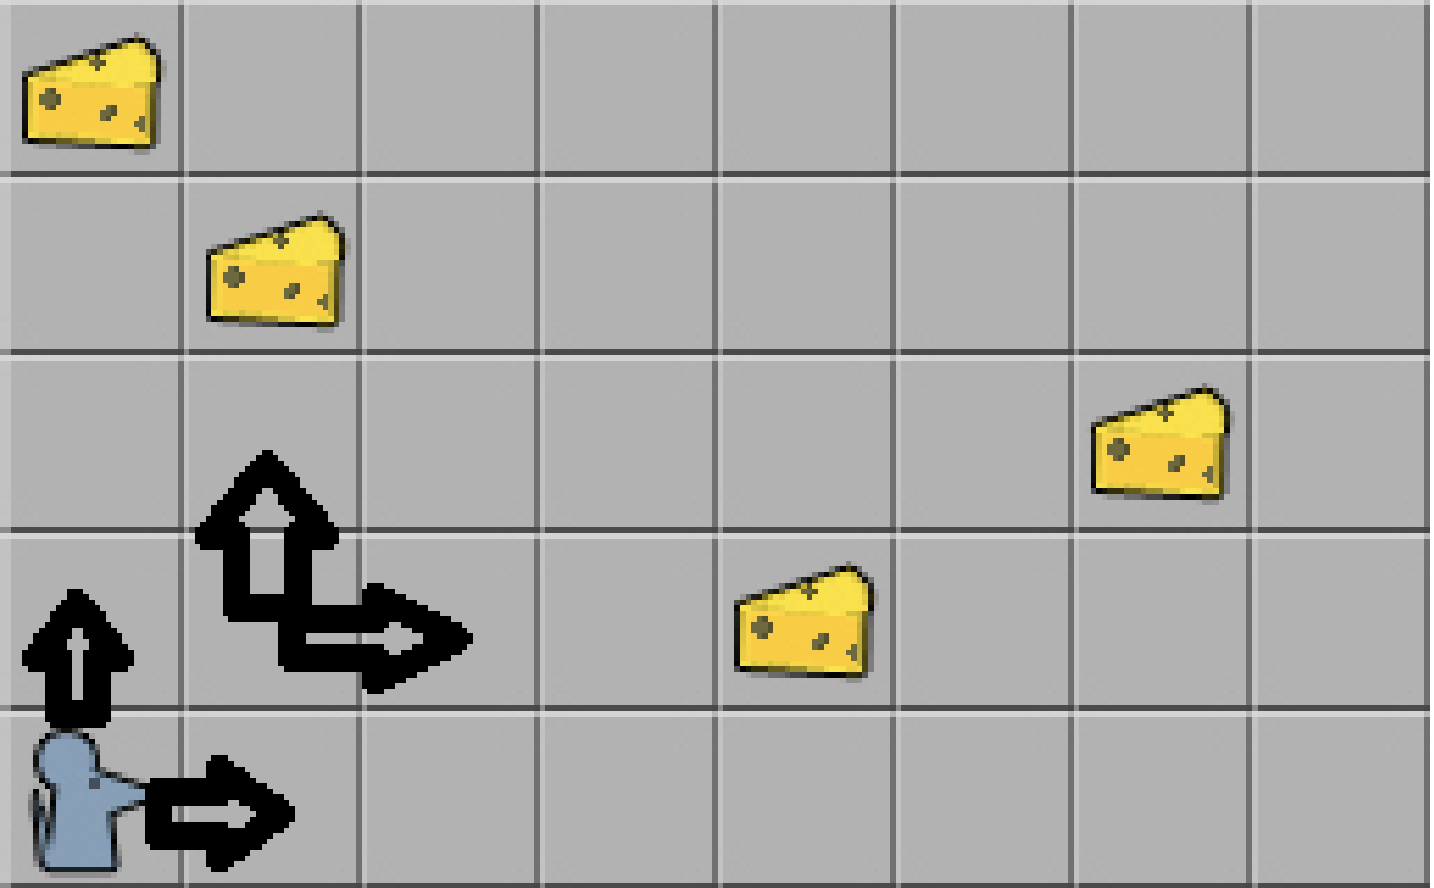
\includegraphics[width=.6780\linewidth]{moses.png}
\end{figure*}

Being a mouse and all, Moses wants to gather as much cheese as possible until he
reaches the north-east room of the apartment.

\begin{enumerate}
\item Formulate the problem as a finite horizon decision problem: Define the state space,
the action space and the cumulative cost function.
\item What is the horizon of the problem?
\item How many possible trajectories are there? How does the number of trajectories
behaves as a function of $N$ when $M = 2$? How does it behave as a function of $N$
when $M = N$? please note that you don't need to calculate the exact number of states, you can give the order number (this also apply to the rest of this question).
\item Aharon, Moses's long lost war-buddy woke up confused next to Moses and decided
to join him in his quest (needless to say, both mice suffer the same rare head injury). 
\begin{enumerate}[label=(\alph*)]
\item Explain what will happen if both mice ignore each other's existence and act
'optimal' with respect to the original problem.
\item Assume both mice decided to coordinate their efforts and split the loot. How
many states and actions are there now?
\item Now their entire rarely-head-injured division has joined the journey. Assume
there's a total of K mice, how many states and actions are there now?
\end{enumerate}
\end{enumerate}

\subsection{Question 3: Language model\protect\footnote{Question taken from ``046194 - Learning and Planning in Dynamical Systems'' by Shie Manor\textcopyright}}
In the city of Bokoboko the locals use a language
with only 3 letters ('B','K','O'). After careful inspection of this language, researchers have
reached two conclusions:
\begin{enumerate}[label=(\alph*)]
\item Every word starts with the letter 'B'.
\item Every consecutive letter is distributed only according to the previous letter as follows: 
\begin{figure*}[ht!]
  \centering
  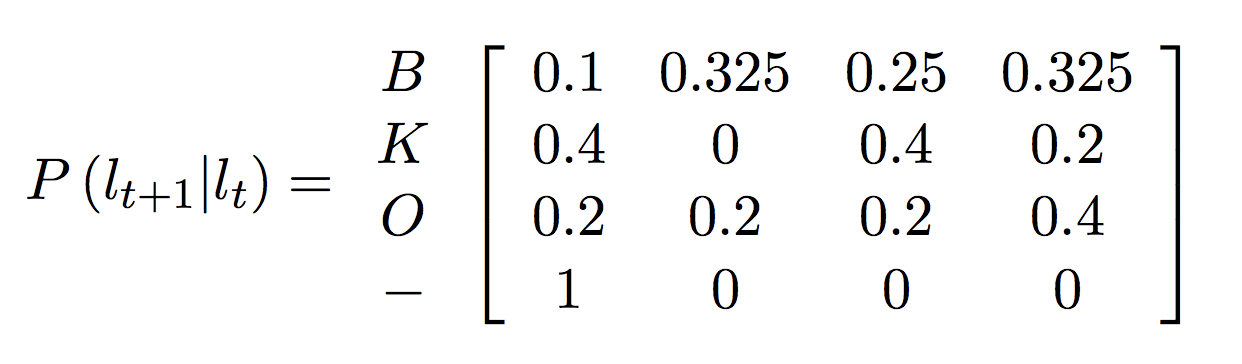
\includegraphics[width=.6780\linewidth]{mat.png}
\end{figure*}
\end{enumerate}




Where '-' represents the end of a word. For example, the probability of the word
'bko' is given by 0.325 * 0.4 * 0.4 = 0.052.

\begin{enumerate}
\item Find the probability of the following words: 'Bob', 'Ok', 'B', 'Book', 'Booook'
\item We wish to find the most probable word in the language of length K.
\begin{enumerate}[label=(\alph*)]
\item Formulate the problem as a finite horizon decision problem: Define the state
space, the action space and the multiplicative cost function.
\item Bound the complexity of finding the best combination.
\item Find a reduction from the given problem to an analogous problem with additive
cost function instead.
\item Explain when each approach (multiplicative vs. additive) is preferable.
Hint: Think of the consequence of applying the reduction on the memory representation
of a number in a standard operating system.
\item  Write a code in Python which finds the most probable word of a given size using
dynamic programming. What is the most probable word of size 5?
\end{enumerate}
\end{enumerate}

\subsection{Question 4: Minimum mean cost cycle}
The following graph describes a 	Deterministic Decision Processes with an initial state $s=A$.

\begin{figure*}[ht!]
  \centering
  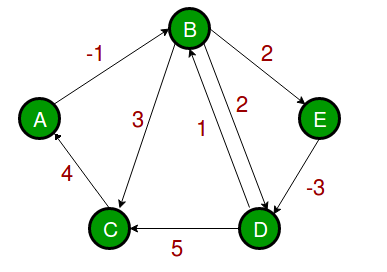
\includegraphics[width=.6780\linewidth]{graph for min mean cost cycle.png}
\end{figure*}




\begin{enumerate}
\item Calculate $d_i(v)$ for every $i\in \{0,\dots,n=5\}$ and every $v\in \{A,B,C,D,E\}$.
\item Use Karp's theorem to find the cost of the minimum mean cost cycle.
\item What is the optimal average cost of this DDP?
\end{enumerate}


% \newpage
% \section{Programing}

% \subsection{Question 1: MNIST}
% Given the MNIST dataset which consists of $28\times28$ image showing a handwritten digit from 0 to 9, and corresponding labels stating what digit the image shows, the goal is to learn a classifier that predicts the class (label) of several test-set inputs. 

% \begin{figure}[h!]
% 	\caption{Example for MNIST images}
% 	\centering
% 	\includegraphics[width=6cm,height=6cm,keepaspectratio]{mnist}
% \end{figure}

% You are provided with training script ``mnist.py''. The script trains a simple logistic regression model to solve the task at hand. For it to work, you'll need to implement missing functionality.
% \begin{enumerate}
% 	\item Implement the training and evaluation loop currently marked as ``TODO'' comments in the code. Use the already defined model and dataset. Make sure you report the loss on the training set each batch and the accuracy on the evaluation set at the end of training.
% 	\item Find a better optimization configuration that works well (learning rates, mini-batch size, no. of epochs and so on). You are provided with some starter configuration options for SGD. However, more options are possible and the values provided are not necessarily optimal. With a better choice of parameters, you will converge much faster and achieve better accuracy. \\ \\
% The new configuration should result \textbf{faster} (in terms of \#epochs) convergence. \textbf{Optional:} You are not limited to SGD and are encouraged to try other optimization methods, see PyTorch optim package.
%     \item Train a deeper model by introducing a ReLU non-linearity and another linear layer. The size of the hidden layer should be 500.
% \end{enumerate}

% Submit your modified code (for each part), plots of the training loss curve comparing all the parts together, the accuracy you achieved on the test set%and a path to the model you trained on nova
% . \\ \textbf{NOTE:} Evaluate the different configurations for at least 100 epochs.

% \newpage

% \subsection{Question 2: OpenAI Gym}

% In this question you will learn how to use OpenAI Gym by training an agent using random search on the ``CartPole-v0'' environment. The problem consists of balancing a pole connected with one joint on top of a moving cart. The only actions are to add a force of -1 or +1 to the cart, pushing it left or right.

% \begin{figure}[h]
% 	\caption{CartPole environment}
% 	\centering
% 	\includegraphics[width=6cm,height=6cm,keepaspectratio]{cartpole}
% \end{figure}

% \begin{enumerate}
% \item Familiarize yourself with OpenAI Gym by going over the short introduction available here: \url{https://gym.openai.com/docs/}. You should be able to understand how to load an environment, perform an action and the observations returned.

% \item In CartPole's environment, each step returns a 4-dimensional observation vector representing information such as the angle of the pole, cart position and so on. Given that observation, your agent will need to act: move left or right. \\ \\
% Implement the following agent: Given a 4-dimensional observations, $o_t \in \mathbb{R}^4$, define the following agent:
% \begin{equation}
%     a_t = agent(o_t, w) = 
% \begin{cases}
%     1, 		& \text{if } o_t*w \geq 0\\
%     -1,     & \text{otherwise}
% \end{cases}
% \end{equation}
% Where $w \in \mathbb{R}^4$ is a vector of weight, each weight corresponding to one of the observations. Initialize the weights randomly between [-1, 1]. 

% \item Evaluate your agent by running an \text{\bf episode} of the environment. An episode ends when the pole drops or 200 steps have passed. The score of your agent, should be the accumulated reward for all steps in the episode.

% \item Train your agent using \text{\bf{random search}}. This is done by sampling different weights multiple times and greedily choosing the weights who scored the highest reward. You should sample at least $10000$ times. 

% \item Evaluate the suggested random search scheme. Run the search for 1000 times and report for each search the number of episodes required until the agent reached a score of 200. Plot a histogram of number of episodes required until score 200 and report the average number of episodes.

% \end{enumerate}

% Submit your full training code (agent, episode and random search), the histogram plot and the average number of episodes.

\end{document}